\documentclass[10pt,twocolumn,letterpaper]{article}

\usepackage{cvpr}
\usepackage{times}
\usepackage{epsfig}
\usepackage{graphicx}
\usepackage{amsmath}
\usepackage{amssymb}
\usepackage{algorithm2e}
% Include other packages here, before hyperref.

% If you comment hyperref and then uncomment it, you should delete
% egpaper.aux before re-running latex.  (Or just hit 'q' on the first latex
% run, let it finish, and you should be clear).
\usepackage[breaklinks=true,bookmarks=false]{hyperref}

\cvprfinalcopy % *** Uncomment this line for the final submission

\def\cvprPaperID{****} % *** Enter the CVPR Paper ID here
\def\httilde{\mbox{\tt\raisebox{-.5ex}{\symbol{126}}}}

% Pages are numbered in submission mode, and unnumbered in camera-ready
%\ifcvprfinal\pagestyle{empty}\fi
\setcounter{page}{4321}
\begin{document}

%%%%%%%%% TITLE
\title{Playing Coinrun with Q-Learning}

\author{Sunil Kumar\\
Uvic\\
BC, Canada\\
{\tt\small sunilkumar@uvic.ca}
% For a paper whose authors are all at the same institution,
% omit the following lines up until the closing ``}''.
% Additional authors and addresses can be added with ``\and'',
% just like the second author.
% To save space, use either the email address or home page, not both
}

\maketitle
%\thispagestyle{empty}

%%%%%%%%% ABSTRACT
\begin{abstract}
   We have seen Proximal Policy Optimization (PPO) a improve version of Policy Gradient method of Reinforcement Learning successfully working on environments like Coinrun in the paper "Quantifying Generalization in Reinforcement Learning" \cite{cobbe_quantifying_2018}. The paper explores the effect of known generalization techniques like dropout, batch, etc. and different NN architecture on PPO. As my project, I will be apply Q-learning on the same environment Coinrun and see how good is this technique. More specifically I will be applying a Deep Q-Network (DQN) and its variant with the intention of understanding the strength and weakness of the different Deep Q-Learning techniques. 
\end{abstract}

%%%%%%%%% BODY TEXT 
\section{Introduction}

% Write a brief introduction to what your project goal is and motivations.

In the 1950s, behavioral psychology gave birth to the main idea behind Reinforcement Learning (RL), that all animals learn to perform better in specific tasks if they are given positive rewards after the completion of such tasks \cite{Sutton1988ReinforcementLA}. Keeping this idea in mind, RL has become a new sub-discipline of Artificial Intelligence (AI). RL is different than existing Machine Learning techniques. For example, RL is different then Supervised Learning because the feedback in RL is not complete, and most rewards are delayed, i.e., a reward is given after doing multiple steps instead of each step. It is also not an Unsupervised Learning because the goal of RL is not to find a hidden pattern in unlabeled random data but to maximize the reward solely. Initially, the applications of RL were limited to simple low-dimensional problems. However, with the increase in computational power in the last decade researchers can work on large data-sets.

The current decade has seen rapid growth in Artificial Intelligence. For instance, Google's DeepMind team created the AlphaGo algorithm which won against Lee Sedol during a 5-game tournament in the game of Go \cite{silver_mastering_2016}, setting a new landmark in AI research. Later they developed AlphaGo Zero \cite{silver_mastering_2017} using only Self-Play with RL, which does not use any dataset or human knowledge and it performed better than original AlphaGo. Then, there is OpenAI team (largely funded by Elon Musk) made AI for Dota2\footnote{https://en.wikipedia.org/wiki/Dota\_2} 1v1 in 2017\footnote{OpenAI Dota 2 1v1 Bot, 2017. Https://openai.com/the-international/} which defeated the human world champion. Further, they built OpenAI Five\footnote{OpenAI Five Final, April 2019. https://blog.openai.com/openai-five-benchmark-results/ https://openai.com/blog/openai-five-finals/ https://openai.com/blog/how-to-train-your-openai-five/} which as of 13 April 2019 have won against human world champion team and many other pro teams in a 5v5 game. Also recently, DeepMind came up with AlphaStar \cite{arulkumaran_alphastar:_2019} which is the first AI system to defeat a top professional player at the game of StarCraft II \footnote{https://en.wikipedia.org/wiki/StarCraft\_II\:\_Wings\_of\_Liberty}. I have a passion for games and Computer Science, and the research on AI for games has really pumped me up. 

Currently, RL is a very hot field of study. Hence, many RL based environments have been created to help researchers develop and compare their RL algorithms. For example, StarCraft II Learning Environment \cite{vinyals_starcraft_2017}, Boomarman \footnote{Pommerman: AI research into multi-agent learning, 2018. Https://www.pommerman.com/}, OpenAI's Gym, Atari 2600 Games \cite{mnih_playing_2013,mnih_human-level_2015} etc. Coinrun is one of such environment developed by OpenAI's team in late 2018 as part of their experiment for the paper 'Quantifying Generalization in Reinforcement Learning' \cite{cobbe_quantifying_2018}. 

The goal of my project will be to understand how different Q-Learning techniques are actually works by implementing as many as I can before the project deadline. It will be interesting to understand the reasons behind OpenAI's decision to use Policy gradient methods instead of Q-Learning. I will be taken help from different papers to apply Q-Learning techniques on Coinrun environment. For example, DQN was applied to play Atari games \cite{mnih_human-level_2015} and a standard way of applying DQN was purposed later \cite{applyDQN}.

\section{Theoretical Background}
\label{rl}

\begin{figure}[h]
   \centering
    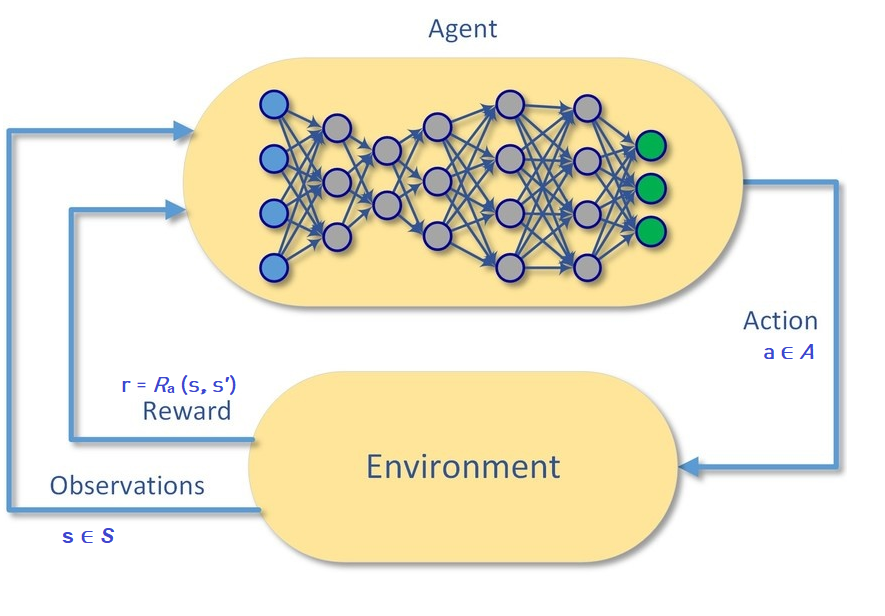
\includegraphics[width=0.50\textwidth]{images/agent-env-intraction3.png}
    \caption{An illustration of the interaction between the agent and the environment
through states/Observation, actions and getting reward based on the action. Note when the agent is a Neural network it becomes Deep Reinforcement Learning }
    \label{fig:basic}
\end{figure}

 Reinforcement Learning problems are commonly expressed using Markov Decision Processes (MDP). A MDP is a model consisting of a set of all possible states S, all possible actions $ A $ and a reward function $ R _ { a } \left( s , s ^ { \prime } \right) $ for each possible state transition $ T $ . States are memory-less and contain all relevant information about the past (also known as the Markov Property) \cite{Sutton1988ReinforcementLA}.

Reinforcement learning deals with how an agent finds an optimal policy, $\pi (s, a ) \in \Pi $, i.e., a series of action $ a $ at state $ s $, which maximize the expected cumulative reward

\begin{equation} 
\label{eq:1}
\sum _ { t = 0 } ^ { n } \gamma ^ { t } R _ { a } \left( s _ { t } , s _ { t + 1 } \right) 
\end{equation}
 

by interacting with the environment, where $R _ { a }$ is the reward received for action $ a $, which happened at time step $ t $ and the state changed from $ s $ to $ s^ { \prime } $ . $ \gamma $ is a parameter, $ 0 \leq \gamma \leq 1 $ called the discount rate \cite{Sutton1988ReinforcementLA}. The concept of discounted reward is similar to the concept of money in finance i.e. getting 100 \$ tomorrow are more valuable than getting 100 \$ one year later. Note that each time the agent interacts with the environment, we obtain a data point $<s,a,r,s^{\prime} > $.

Many deep learning based solutions have been proposed to find the best policy for MDPs, such as Monte Carlo search \cite{browne_survey_2012},  Policy Iteration \cite{thomas_bias_2014} and Q-learning \cite{watkins_q-learning_1992}. Let us see a few of these in detail.

\subsection{Deep Reinforcement Learning}
\label{deepRL}

Deep Learning \cite{lecun_deep_2015} is a technique of using a Neural Network model to solve a complex problem like speech recognition, visual object recognition and so forth. When Deep Learning is combined with reinforcement learning, then it is called Deep Reinforcement Learning \cite{francois-lavet_introduction_2018}.

The two major types of Deep RL are Model-based learning and Model-free learning. In Model-based learning, the agent is required to learn a model which describe how the environment works from its observations and then plan a solution using that model. Model-free learning is when an agent can directly derive an optimal policy from its interactions with the environment without needing to create a model beforehand. The most common methods for Model-free learning are Q - Learning and Policy Gradient. Both of these methods have many variants available today like DQN, DDQN, TRPO, PPO, TRPPO, etc.

\subsubsection{Q-Learning \footnote{ Some part of the text is taken from https://flyyufelix.github.io/2017/10/12/dqn-vs-pg.html}} 


First of all, Q function is defined as the expected value of the sum of future rewards by following policy $ \pi $.
\begin{equation} 
\label{eq:q_function}
Q^{\pi}(s, a)=E\left[R_{t}\right]
\end{equation}

Here $R_{t}=r_{t}+\gamma r_{t+1}+\gamma^{2} r_{t+2}+\ldots$ .
The idea of Q Learning is that if we have a good approximate of Q function for all state and action pairs, we can obtain the optimal policy $\pi^{*}(s)=\operatorname{argmax}_{a} Q(s, a)$. 

Now we have data points $<s,a,r,s^{\prime} > $ to approximate Q function. The Bellman equation will help us relates the Q functions of consecutive time steps
\begin{equation} 
\label{eq:bellman}
Q^{{\pi}^*} ( s , a ) = r + \gamma \max _ { a ^ { \prime } } Q \left( s ^ { \prime } , a ^ { \prime } \right)
\end{equation}

So, bellman equation become our target value and our predicted value will be the $Q(s,a)$ (initially random values). This give us the loss function
\begin{equation} 
\label{eq:qloss}
L=\left[r+\gamma \max _{a^{\prime}} Q\left(s^{\prime}, a^{\prime}\right)-Q(s, a)\right]
\end{equation}

For simple environments, we do tabular Q-Learning where we use a table $ S X A $, which can be initialized with random values and as the agent's interaction with the environment we can update the estimated value of Q function in that table. This process is also known as Boltzmann exploration. But for a problem with larger state-action search space, we use a Deep Neural Network to approximate the Q function. This is called Deep Q-Network i.e. DQN. I am hoping of playing Coinrun with the native DQN or with a slightly improved version of it like Double DQN or Dueling DQN.

\subsubsection{Policy Gradient}
\label{qlearn}

While the goal of Q Learning is to approximate the Q function and use it to infer the optimal policy $\pi^{*}(s)=\operatorname{argmax}_{a} Q(s, a)$, Policy Gradients (PG) seeks to directly optimize in the policy. By using a Deep Neural Network to directly predict probabilities of actions at a particular state. To come up with the best policy, we choose a set of actions and then adds randomness to those actions. If the new total output reward is better, then we increase the likelihood of those actions. The same thing can be translated from the improved loss function of PG:-

\begin{equation} 
\label{eq:pgloss}
L^{P G}(\theta)=\hat{E_{t}}\left[\log \pi_{\theta}\left(a_{t} | s_{t}\right) \hat{A}_{t}\right]
\end{equation}

Here $\hat{A_t}$ is the advantage function which defined as the difference of two terms Discounted Reward (Eq. \ref{eq:1}) and Baseline Estimate of reward at a point. So, +ev $\hat{A_t}$ mean we have collected higher reward than expected and hence the loss function help us increase the action probabilities of those actions and vice-versa. Hence, the Advantage term is used as the “Critic” to evaluate the goodness of an action hence corresponding gradient estimation method is known as Advantage Actor-Critic (A2C). Bite here the policy network acts as the “Actor”.

 Generally, an environment has multiple possible actions with one ultimate final goal for which reward is given. This causes a problem known as Sparse Rewards System \cite{sparse_reward} which arises mainly due to too many actions needed before receiving the reward, which makes it really hard by just doing random action to get a successful reward with a +ev gradient to decent toward the optimal solution. To tackle this sparse reward system, we do reward shaping (manually design rewards for some +ev actions) which does make it easy to converse to a solution. But there are downsides of reward shaping also. 1st, it's a custom process it has to be re-done for every new environment; for example, all Atari games require separate personalized optimal Reward Shaping. So this is also not scalable.
 
 2ndly, Reward Shaping also gives raises to "The Alignment Problem" \footnote{https://ai-alignment.com/the-reward-engineering-problem-30285c779450} in which agent will find a lot of ways of getting the small useless reward without doing the ultimate goal. And lastly, this reward shaping is optimized based on human behaviors which might not be optimal for many environments for example in the game of Go where we actually want to surpass human knowledge.

\section{Contribution of the paper "Quantifying Generalization in Reinforcement Learning" \cite{cobbe_quantifying_2018}}

\begin{enumerate}
    \item New environments for experimenting for other researchers i.e. Coinrun and Coinrun-platform.
    \item They showed that the number of different training levels required for a good generalization is much larger than the number used by prior work on training in RL. Gave a metric based on experimenting with 3 different environments.
    \item Generalization metric using the Coinrun environment. This could help future researchers who plan to use Coinrun to setup there technique accordingly. 
    \item They evaluate the impact of 3 different convolutional architectures (Nature-CNN \cite{mnih_human-level_2015}, IMPALA \cite{IMPALA} & IMPALA Large ) and methods of generalization including Dropout, L2 regularization, Data augmentation, batch normalization, and Stochasticity.
\end{enumerate}


\section{Contributions of this project}

Project Goal: It's my first Reinforcement Learning implementation so I decided to start from scratch to have an intimate understanding of every step of the process of a DQN algorithm. I will be using Pytorch instead of tensorflow which is used by the paper.

I am using Coinrun environment which seems to have a different interface than other Arcade Learning Environments like OpenAI gym. Turn out Coinrun is a vector environment which means that it takes a list of inputs and return a list of states and rewards. I find out that this kind of environment can be helpful in policy gradient methods (like PPO2 method in the paper) for faster stepping and faster batch learning but not really usable for DQN. After searching a bit, In issues section, I get my hands on a scalar adapter class which helped me wrap the vector environment and use it as a Scalar environment with minor limitations. In DQN we do one step at a time so Scalar environment was needed. Note: maybe vector version can be used to fill the initial experience replay buffer fast but I did not try this method because it normally takes only 30 to fill up Experience Replay Buffer of size 10,000  to start the training with.

Coinrun is able to create levels with varying complexity. But for our experiments, we will be using fixed levels as showing in Fig. \ref{fig:simplecoinrun} and \ref{fig:simplecoinrun2}. This should significantly reduce training time. If time permits and everything goes well then we will run the same for random 5 levels or more. 

\begin{figure}[h]
   \centering
    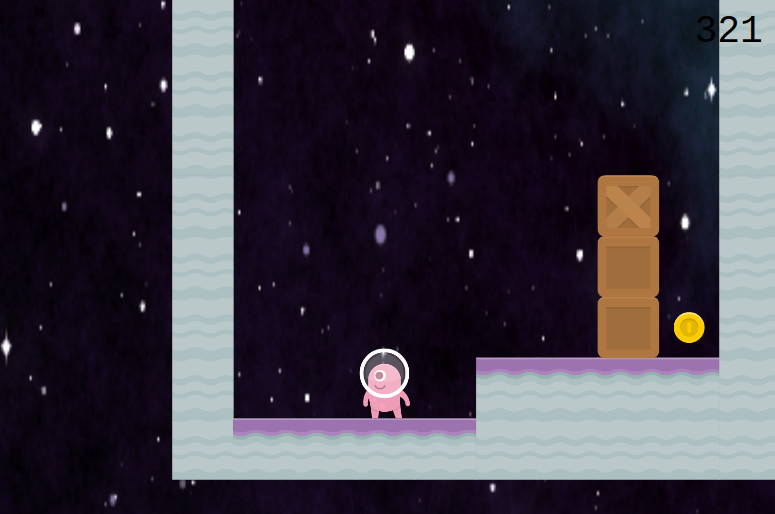
\includegraphics[width=0.50\textwidth]{images/simple_seed8.png}
    \caption{One is very simple level can be recreated using '--num-levels 1 --set-seed 8' }
    \label{fig:simplecoinrun}
\end{figure}

\begin{figure}[h]
   \centering
    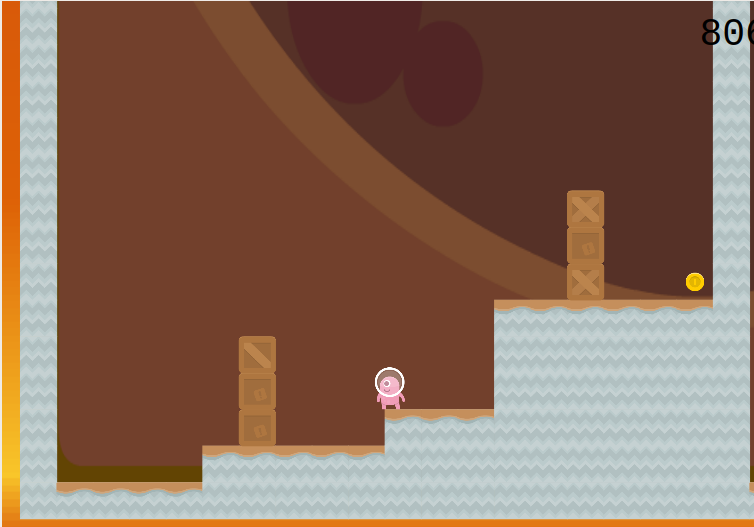
\includegraphics[width=0.50\textwidth]{images/med_seed0.png}
    \caption{Another simple a little larger Level can be recreated using '--num-levels 1 --set-seed 0' }
    \label{fig:simplecoinrun2}
\end{figure}


\subsection{Basic DQN}

Basic DQN algorithm is shown in Figure \ref{fig:dqn_algo}:-

\begin{figure}[h]
   \centering
    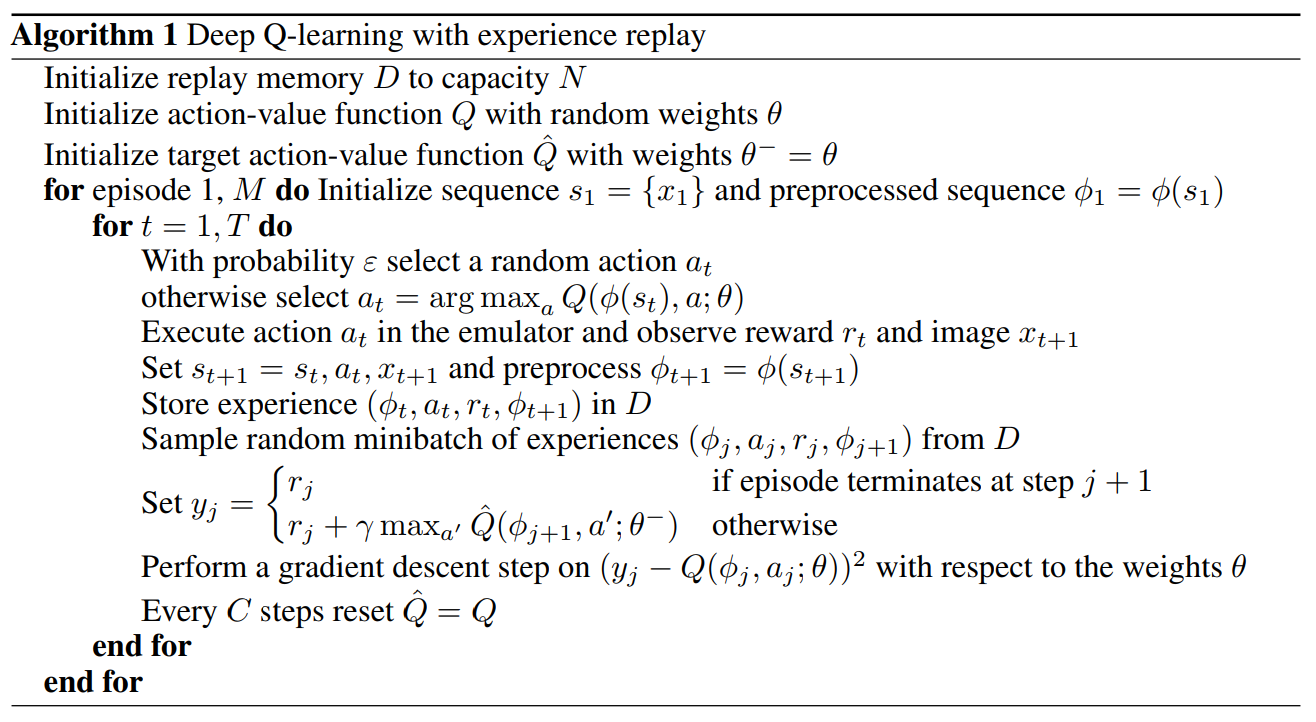
\includegraphics[width=0.50\textwidth]{images/dqn.png}
    \caption{Basic DQN Algo. with Target network: Q-function that is fixed over many (∼ 10, 000)
time-steps}
    \label{fig:dqn_algo}
\end{figure}

Points should be noted for Basic DQN:-
\begin{itemize}
  \item Input to the Q-function Neural Network is the observation state of the game in the form of a state image
  \item Output of Q-function Neural Network is a 1-D array estimating reward earned for each possible actions given the current state.
  \item There are two Neural Networks Q-function and Target Q-function which is same as Q-function but frozen for 10,000 timestamps
\end{itemize}


We going to use a simple CCN architecture as shown in Figure Below. Which is very similar to the one used by Deepminds to play Atari games with 3 Conv. layers and 2 linear layers wrapped by relu activation functions.

\centerline{
   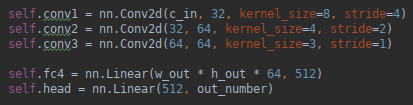
\includegraphics[width=0.50\textwidth]{images/network1.png}
}
% \begin{figure}[h]
%   \centering
%     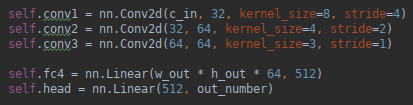
\includegraphics[]{images/network1.png}
%     \caption{Simple CNN with 3 Conv. layers and 2 linear layer wrapped by relu function }
%     \label{fig:network}
% \end{figure}

Flow Diagram of DQN Algo. has been shown in figure \ref{fig:dqnflow}. Note the learning starts after the minimum experience have been collected in the replay buffer.

\begin{figure}[h]
   \centering
    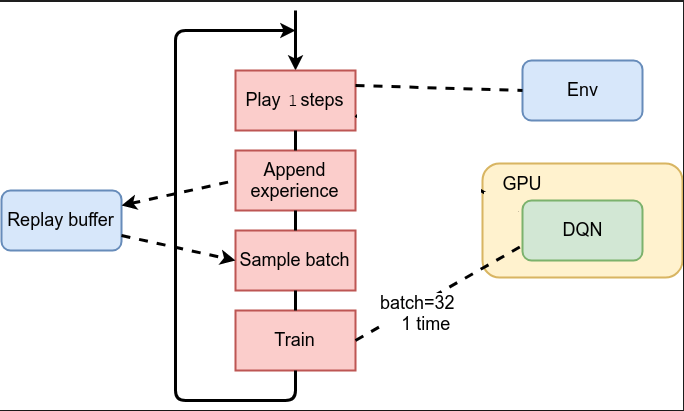
\includegraphics[width=0.50\textwidth]{images/dqnflow.png}
    \caption{Flow diagram of DQN }
    \label{fig:dqnflow}
\end{figure}

Performance of the agent, when trained on simple levels, can be seen in Figure \ref{fig:simpledqnoutput}. We can see that training further than 300 episodes not really provide any progress. It was observed that early optimal point was never reached again hence early stopping the training can be beneficial. we will also see that the default reward system does not provide any use-full information about the nature of progress made by the system. To resolve this issue we will be using custom reward shaping.

\begin{figure}[h]
   \centering
    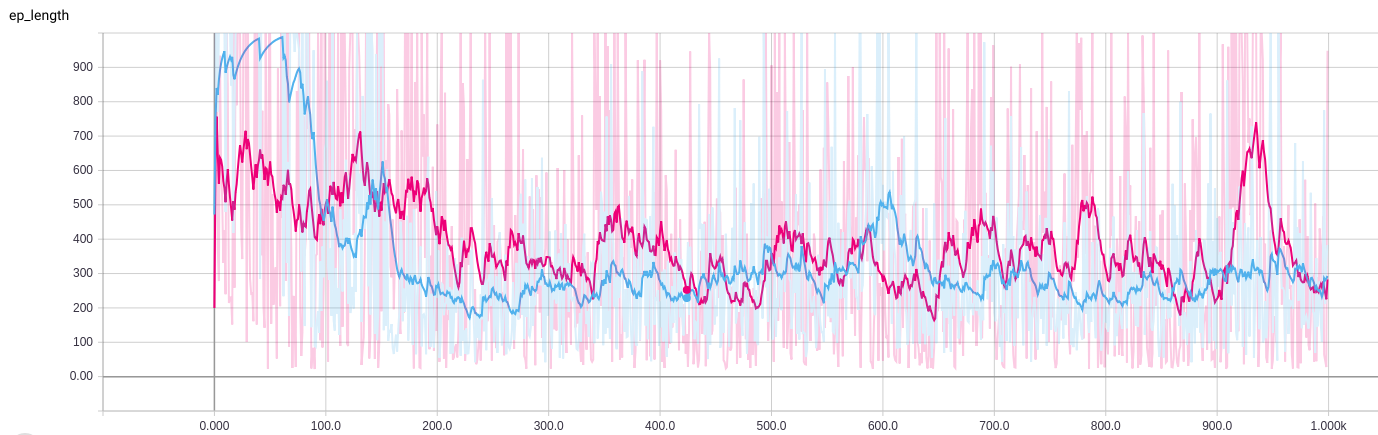
\includegraphics[width=0.50\textwidth]{images/DQNlength.png}
    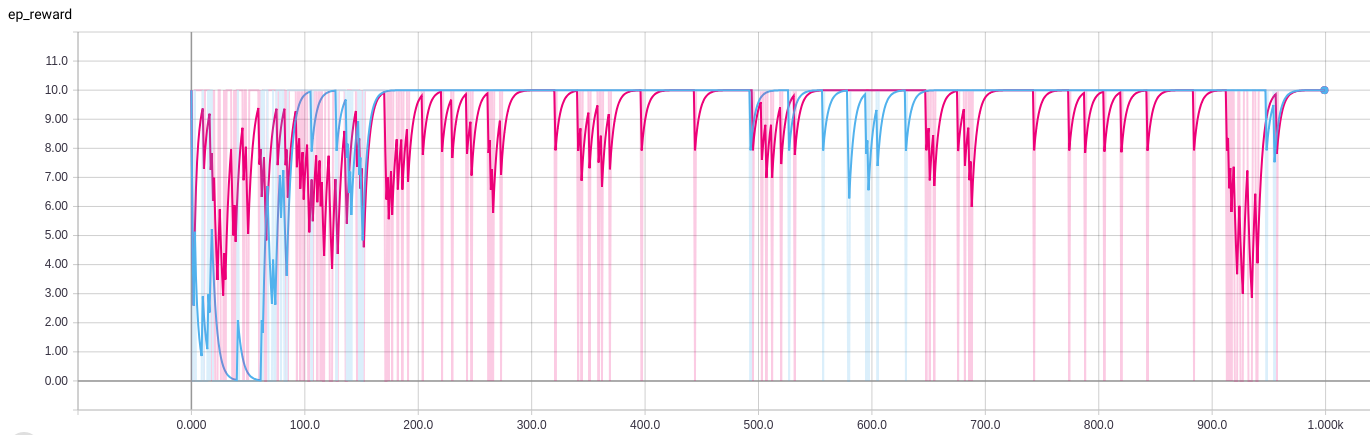
\includegraphics[width=0.50\textwidth]{images/DQNreward.png}
    \caption{Agent's performance with Simple DQN on 2 simple levels}
    \label{fig:simpledqnoutput}
\end{figure}


\subsubsection{Reward Shaping}

Custom Reward Shaping can help give better results in Spare Reward Settings such as Coinrun environment where we have only one reward i.e. 10 points for collection the coin (Section \ref{qlearn}). Different rules for reward shaping can be used to get better results. Following custom reward shaping have been implemented by me in the code:-

\begin{itemize}
    \item Agent will be awarded -1 reward for each timestamp where he did not receive any other reward. this will motivate the agent to do an action which yields positive rewards.
    \item Award for obtaining the coin set to 1000 instead of 10.
    \item If Agent's action did not change the state of the environment then it is awarded -2. this will motivate the agent to perform impact-full actions.
    \item All levels start with an agent on the left and coin at the far right side of the level. Hence performing a forward jump can resolve many obstacles and gets the agent near to the reward hence. action 4 (forward jump) will be awarded 1 reward.
    \item death by any mean will result in -800 rewards. 
\end{itemize}

A graph in Figure \ref{fig:Num1Seed8_1000} show the impact of applying custom reward shaping on DQN performance. We can clearly see reward shaping help in quick conversion of the network to an optimal policy with a positive impact on overall performance.

\begin{figure}[h]
   \centering
    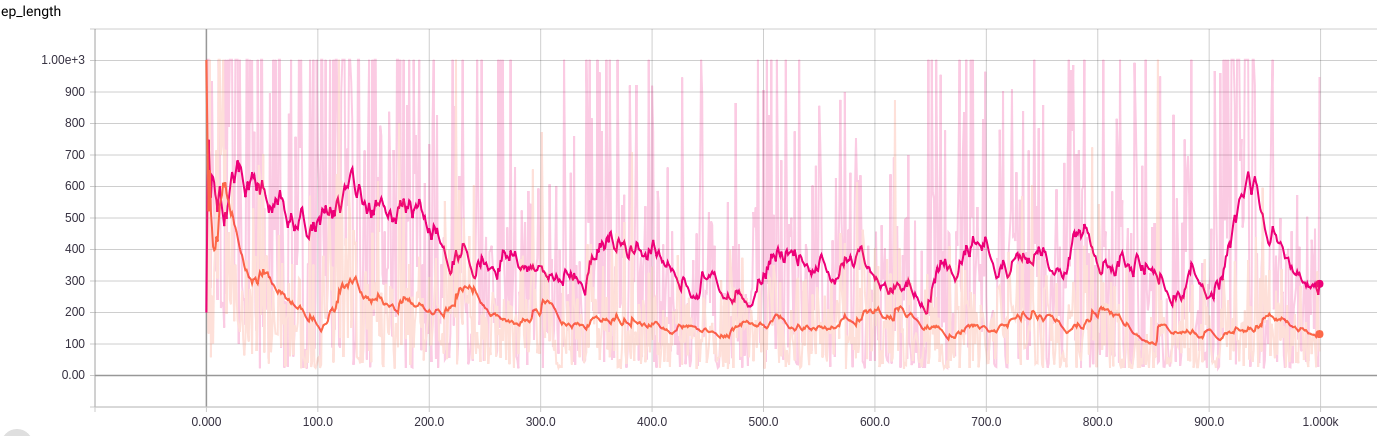
\includegraphics[width=0.50\textwidth]{images/Num1Seed8_1000.png}
    \caption{ Orange with reward shaping enabled. Note as this experiment involve simple level with no agent's death possibility. the length of the episode can be representative of success of the episode }
    \label{fig:Num1Seed8_1000}
\end{figure}


 Challenges faced during this the whole DQN experiment:
\begin{itemize}
    \item how fast should you decay the random movements. finally fixed it to from 1.0 to 0.1 decay over 25000 steps
    \item what should be the associated Adam learning rate. finally fixed it to 0.00025 for rest of the experiments.
    \item how big should be the memory. finally fixed it, start training from 10000 with a maximum of 100000 sizes.
    \item tested batch size 32 and 64. finally fixed with 64 because the reward is sparse and larger batch size have more change to have at-least data point with reward to help progress the network.
    \item writing a bug-free code which writes meaningful logs to track progress.
\end{itemize}

\subsection{Double DQN}

Double DQN method \cite{double_qlearning} is very similar to Simple DQN with minor changes. Double DQN algorithm is shown in Figure \ref{fig:doubledqn}.

% \centerline{
%   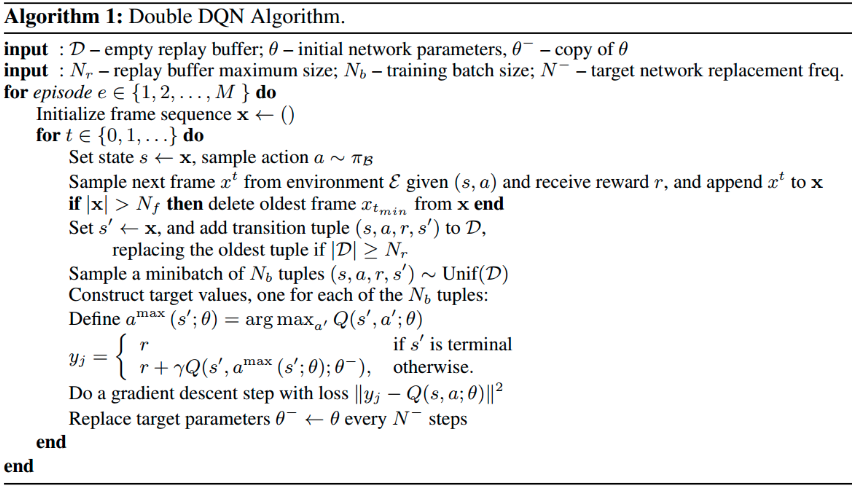
\includegraphics[width=0.50\textwidth]{images/ddqn.png}
% }

\begin{figure}[h]
  \centering
    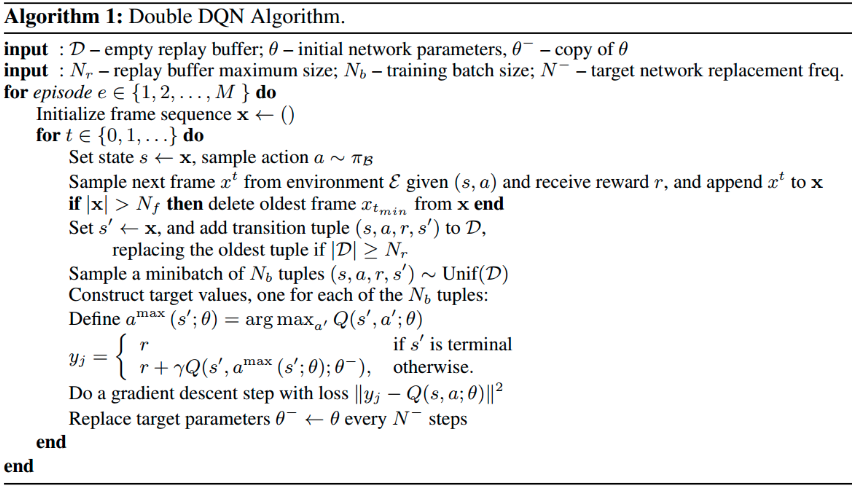
\includegraphics[width=0.50\textwidth]{images/ddqn.png}
    \caption{Double DQN algorithm }
    \label{fig:doubledqn}
\end{figure}

Notice carefully for one major difference between the DQN and Double DQN is that the action is for target Q values are calculated using Q-function and not from the target Q-function. This is done to fix the overestimating the Q-values. Change in the code for this was small because we already have a target network which was not present in the vanilla DQN. The change is shown in Figure \ref{fig:ddqnchange}

\begin{figure}[h]
  \centering
    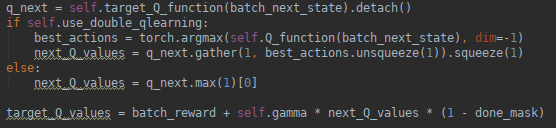
\includegraphics[width=0.50\textwidth]{images/ddqn_change.png}
    \caption{Double DQN algorithm }
    \label{fig:ddqnchange}
\end{figure}

Results with Double DQN compare to DQN with and without reward shaping are displayed in figure \ref{fig:ddqnresults}. The result was taken on one common medium size level. We can clearly see improvement in all factors like the length of the episodes and total episode reward. Further improvement can be seen using custom reward shaping. I figure that reward per timestamp would be a better representation of the performance of the algorithm. So the first graph shows the avg. reward collected per step.


\begin{figure}[h]
  \centering
    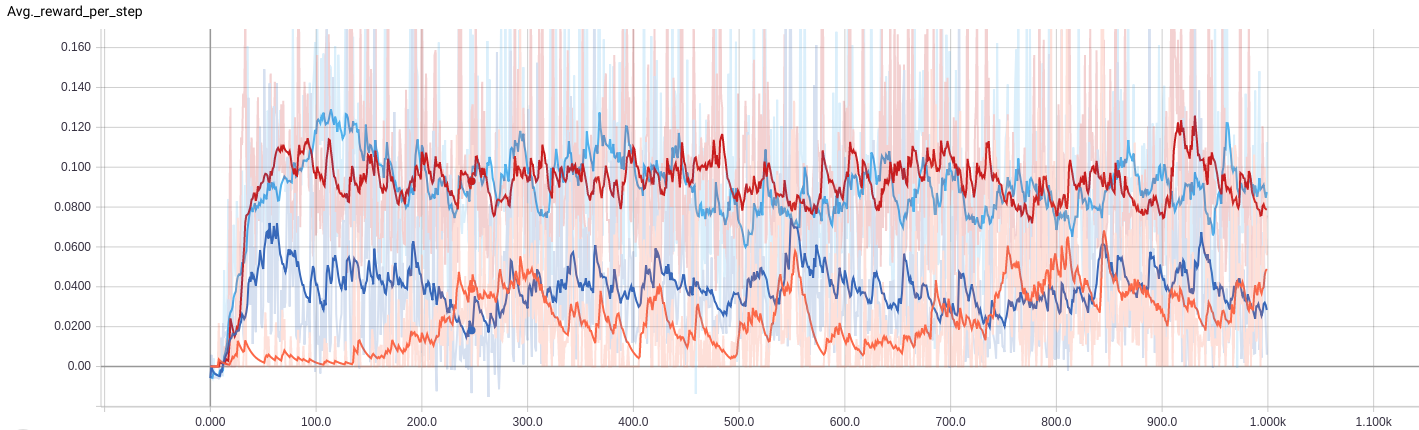
\includegraphics[width=0.50\textwidth]{images/dqnVSddqnAvgRew.png}
    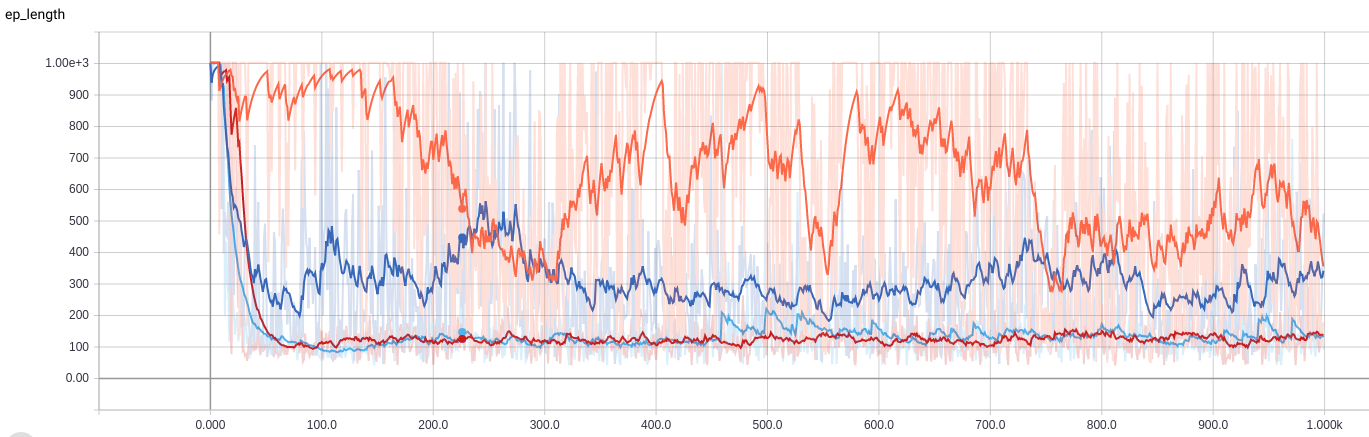
\includegraphics[width=0.50\textwidth]{images/dqnVsDdqnEpLength.png}
    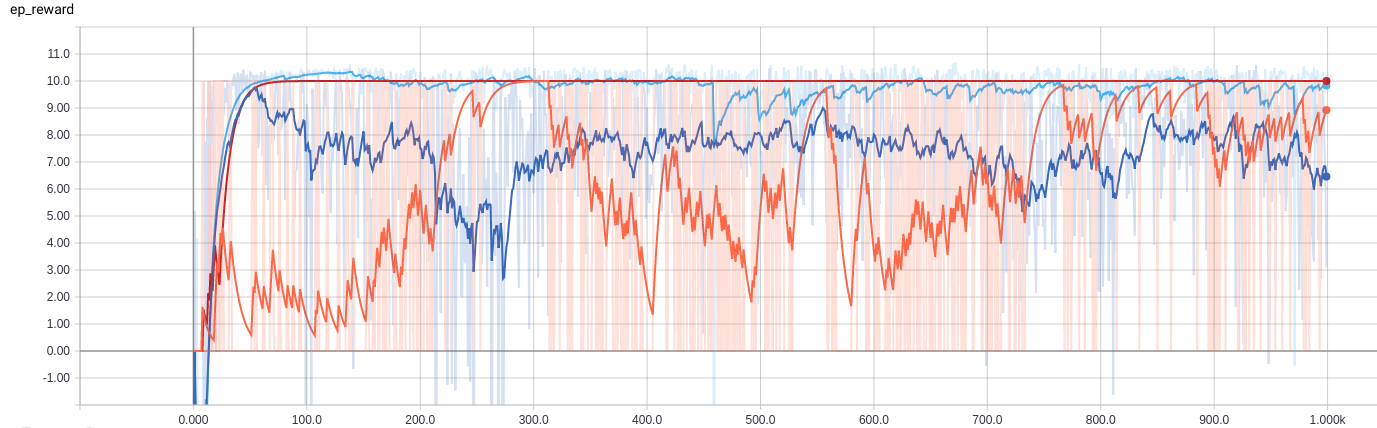
\includegraphics[width=0.50\textwidth]{images/dqnVSddqnEpReward.png}
    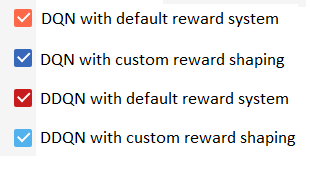
\includegraphics[width=0.30\textwidth]{images/ddqnLegend.png}
    \caption{Comparison of Double DQN vs Simple DQN algorithm with and without custom reward shaping }
    \label{fig:ddqnresults}
\end{figure}


\section{Discussion and future directions}

I found out the DQN for simple levels is able to converge with very few numbers of episodes 100-200. This proof that DQN is sample efficient. But the main problem I faced is that DQN is not able to stay converged to optimal policy for long and start degrading if trained further. Double DQN helped with the needed stability in the DQN and also provide better results. We have also seen custom reward shaping can speed up the time to get an optimal policy in many cases. 

Problem with DQN seems to be its limitation to solve more complex levels. I tried multiple time to train for fixed 5 random levels using DQN and DDQN but none of them are able to get the required performance where we can say it has learned to play decently. Whereas the paper showed PPO able to learn even on the unbounded set of levels.

A further study from my project may include the following:-
\begin{enumerate}
    \item I would love to know the limit of DQN by experimenting with the number of levels for which it can be trained to get decent results.
    \item I would like to implement more variant of DQN and see the impact comparison of such methods like prioritized DQN, distributed prioritized DQN, episodic memory DQN, asynchronous n-step DQN, and multiple DQN. From all of the above, I really want to try out Prioritized DQN when I have time as my own project which according to people really helps.
    \item Impact of different architecture on DQN can be studied through experiments
    \item If any of the above combinations of DQN give stable results then impact of generalization techniques (Dropout, L2 regularization, Data augmentation, batch normalization, and Stochasticity) also can be studied.
\end{enumerate}

As for the weakness in the original method used in the paper, I would have liked to see the impact of LTSM on simple Coinrun environment as part of the paper. Final LTSM node is part of purpose IMPALA Network \cite{IMPALA} and the reason of not using is not clear other than the logic that it probably impacts on the speed negatively. Also, it would be interesting to compare the impact of newly purposed TRPPO algorithm \cite{TRPPO} which claim to be an improvement of the PPO \cite{PPO} technique used in the paper. Also, my experiment with DQN proves that policy gradient methods like PPO are very less sample efficient and hence require a lot more training and computation power then DQN agent. 


{\small
\bibliographystyle{ieee}
\bibliography{egbib}
}

\end{document}
